% Homework 5 - CS386(late submission)
% Russell Miller Winter 2011

\documentclass{article}
\usepackage{anysize}
\usepackage{wasysym}
\usepackage{graphicx}

\marginsize{2cm}{2cm}{2cm}{2cm}

\title{CS386 Homework 5}
\author{Russell Miller}
\date{\today}

\begin{document}

\maketitle

\section{}
\begin{description}
\item[a.]
ERD with cardinality constraints:\footnotemark\\
\footnotetext{ERDs drawn using Dia. http://projects.gnome.org/dia/}
\begin{center}
 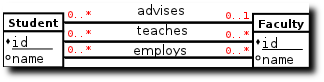
\includegraphics[scale=.8]{1a.png}
\end{center}
Relational Schema for this ERD:
\begin{quote}
Student(\underline{id}, name, advisor) advisor references Faculty.id\\
Faculty(\underline{id}, name)\\
Teachers(\underline{faculty\_id, student\_id}) faculty\_id references Faculty.id, student\_id 
references Student.id\\
Employments(\underline{faculty\_id, student\_id}) faculty\_id references Faculty.id, student\_id 
references Student.id\\
\end{quote}
\end{description}



\end{document}
